
\section{Backtest Study}

In this section we present a backtesting study of a portfolio building with the 10 biggest representative companies in the brazilian market. The list os companies is Ambev S.A. (ABEV3), B3 S.A. (B3SA3), Banco do Brasil S.A. (BBAS3), Banco Bradesco S.A. (BBDC4), Itaúsa S.A. (ITSA3), Itaú Unibanco S.A. (ITUB4), Lojas Renner S.A.(LREN3), Petróleo Brasileiro S.A (PETR4), Vale S.A. (VALE3) and WEG S.A.(WEGE3), in parentheses we have the tickers of each company.  We did a backtest building 2 portfolios with monthly rebalance. One of them was the minimum variance portfolio (MVP), and the other was the risk parity portfolio (RPP) which were obtained solving optimization problems \eqref{eq:MVP} and \eqref{eq:RPP}. Data pertaining to the period between January 2016  and June 2022, was taken from Yahoo Finance (\url{http://finance.yahoo.com}). For rebalancing, the volatilities were calculated, using data from the previous 12 months. 2016 year data was used only for past volatilities calculations. 

One of the main reasons that the MVP has not being used in practice, lies in the fact that, the weights (and consequently the risks) may being concentrated in a few assets. Figure \ref{fig:totalRiskMVP} shows the weight distribution and the risk contribution of stocks during the MVP backtesting study. We note that the MVP concentrates capital in few assets and consequently also concentrates risk in the same assets.

% \begin{figure}[H]
% 	%\begin{adjustwidth}{2.2cm}{2.2cm}
% 	\begin{subfigmatrix}{3}
% 		\subfigure[January]{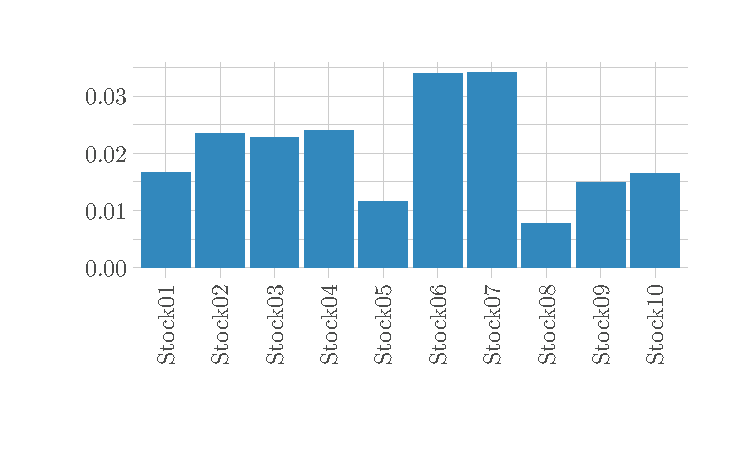
\includegraphics{figures/RiskContribEqual101.pdf}}
% 		\subfigure[February]{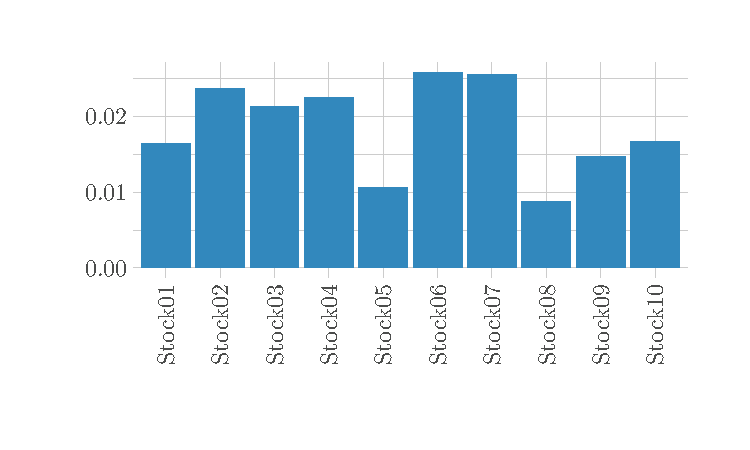
\includegraphics{figures/RiskContribEqual102.pdf}}
% 		\subfigure[March]{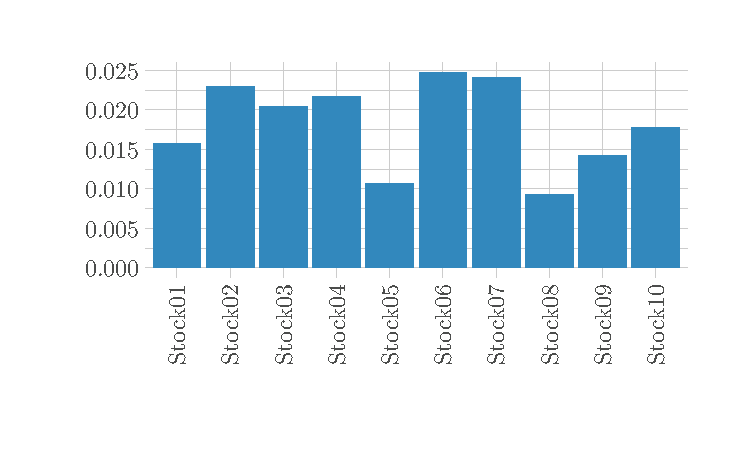
\includegraphics{figures/RiskContribEqual103.pdf}}
% 		\subfigure[April]{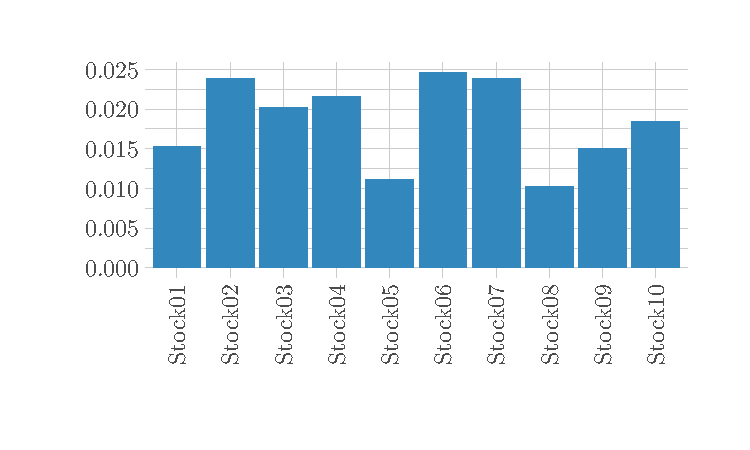
\includegraphics{figures/RiskContribEqual104.pdf}}
% 		\subfigure[May]{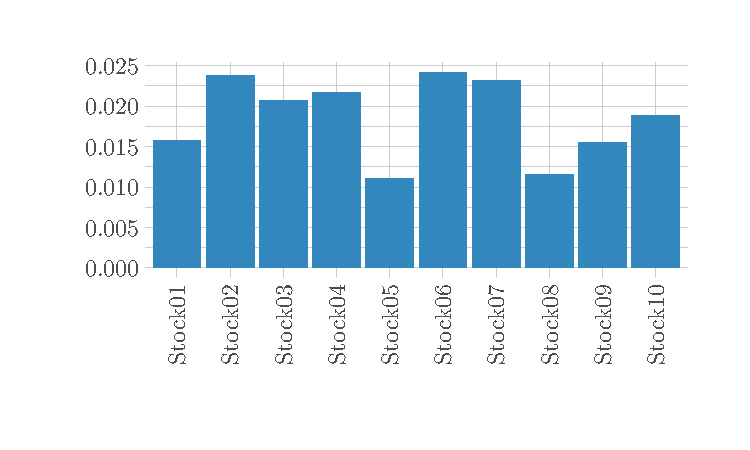
\includegraphics{figures/RiskContribEqual105.pdf}}{}
% 		\subfigure[June]{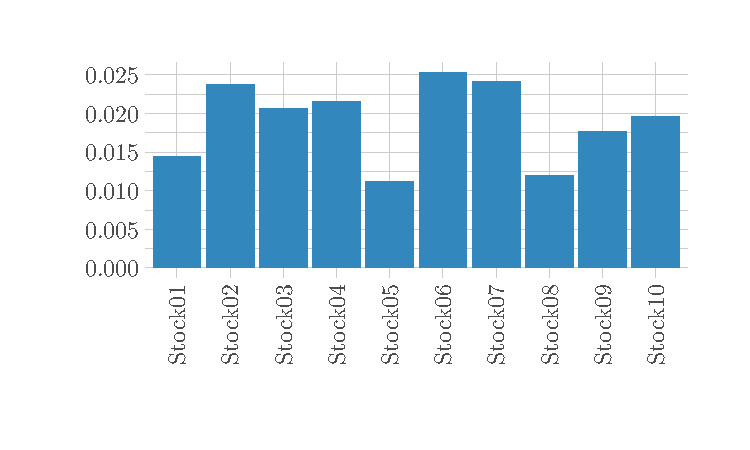
\includegraphics{figures/RiskContribEqual106.pdf}}
% 	\end{subfigmatrix}
% 	\caption{Risk Contributions of EWP.}
% 	\label{fig:condProj1}
% 	%\end{adjustwidth}
% \end{figure}


% \begin{figure}[H]
% 	%\begin{adjustwidth}{2.2cm}{2.2cm}
% 	\begin{subfigmatrix}{3}
% 		\subfigure[January]{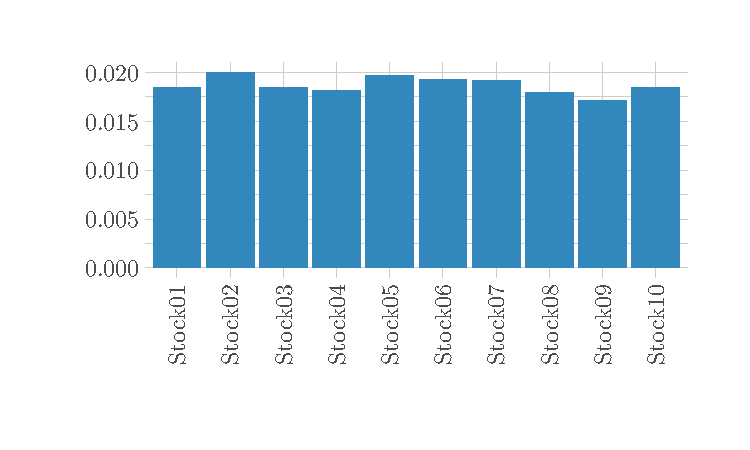
\includegraphics{figures/RiskContrib101.pdf}}
% 		\subfigure[February]{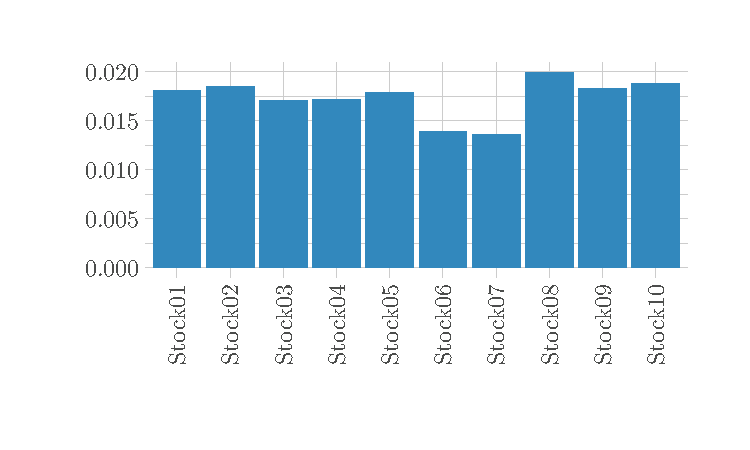
\includegraphics{figures/RiskContrib102.pdf}}
% 		\subfigure[March]{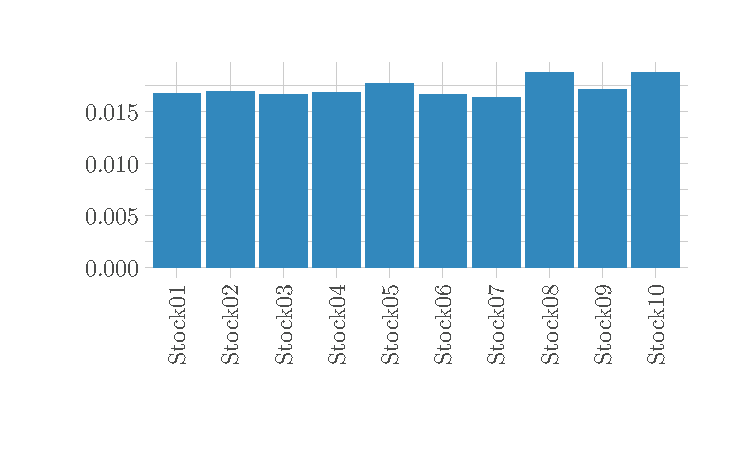
\includegraphics{figures/RiskContrib103.pdf}}
% 		\subfigure[April]{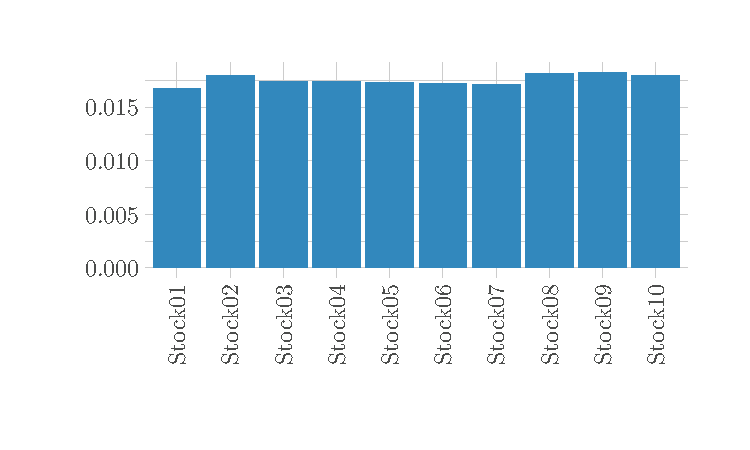
\includegraphics{figures/RiskContrib104.pdf}}
% 		\subfigure[May]{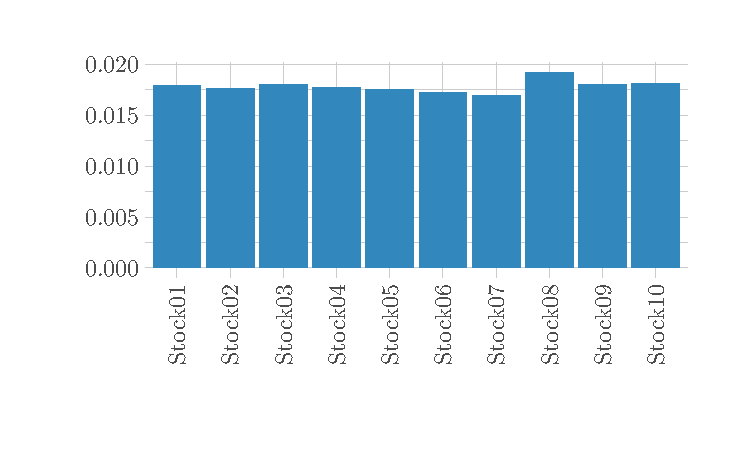
\includegraphics{figures/RiskContrib105.pdf}}
% 		\subfigure[June]{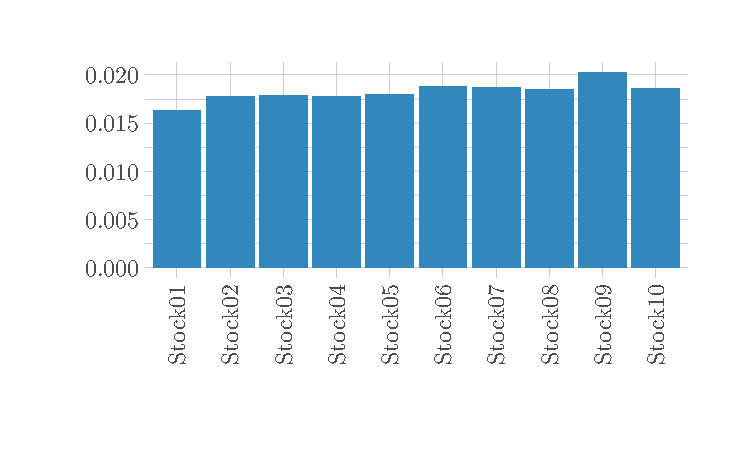
\includegraphics{figures/RiskContrib106.pdf}}
% 	\end{subfigmatrix}
% 	\caption{Risk Contributions of RPP.}
% 	\label{fig:condProj1}
% 	%\end{adjustwidth}
% \end{figure}


\begin{figure}[H]
	%\begin{adjustwidth}{2.2cm}{2.2cm}
	\begin{subfigmatrix}{2}
		\subfigure[Weigths]{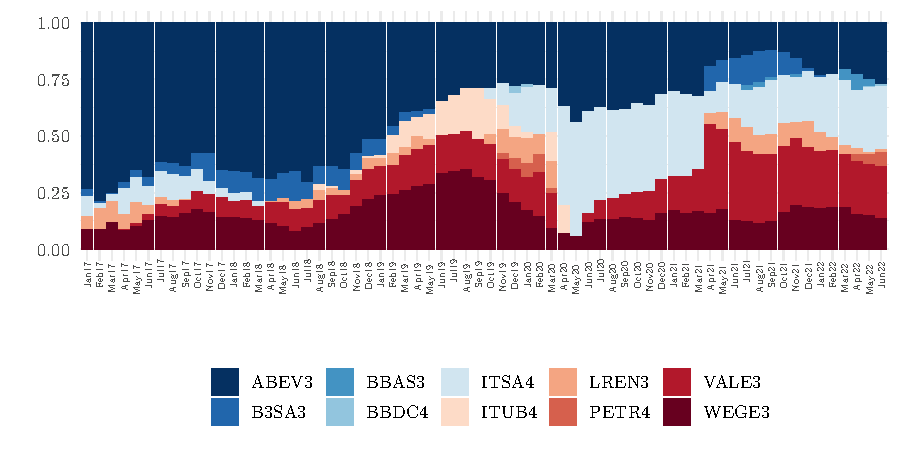
\includegraphics{figures/totalWeigthMVP.pdf}}
		\subfigure[Risks]{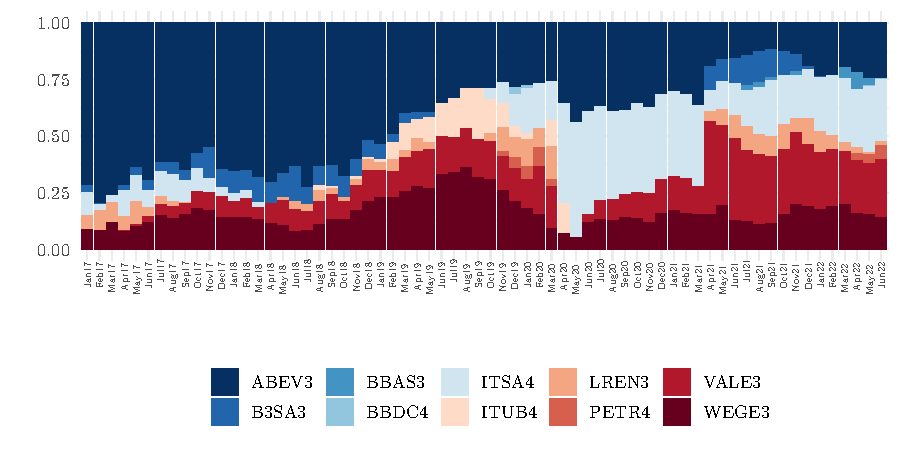
\includegraphics{figures/totalRiskMVP.pdf}}
	\end{subfigmatrix}
	\caption{Monthly distribution of MVP.}
	\label{fig:totalRiskMVP}
	%\end{adjustwidth}
\end{figure}


A RPP has the weights distributed with the purpose of having a risk distribution uniform, Figure \ref{fig:totalRiskPPP} shows the distribution of weights and risks of our backtest study.

\begin{figure}[H]
	%\begin{adjustwidth}{2.2cm}{2.2cm}
	\begin{subfigmatrix}{2}
		\subfigure[Weigths]{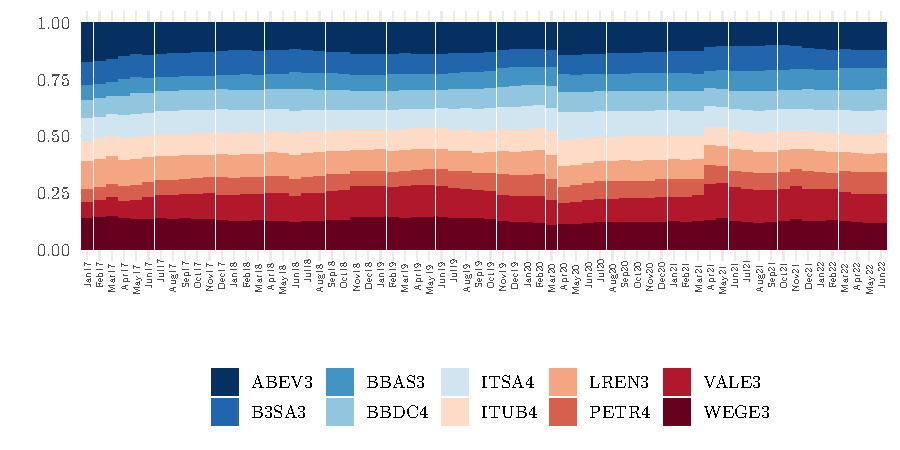
\includegraphics{figures/totalWeigthRPP.pdf}}
		\subfigure[Risks]{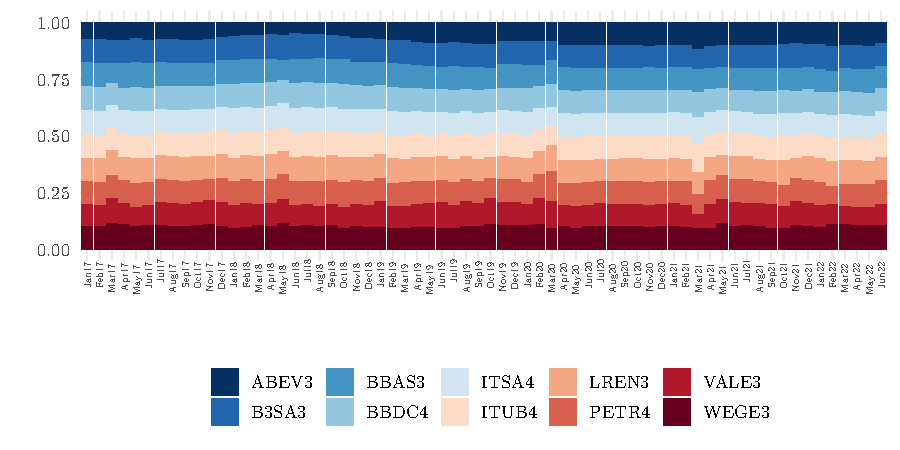
\includegraphics{figures/totalRiskRPP.pdf}}
	\end{subfigmatrix}
	\caption{Monthly distribution of RPP.}
	\label{fig:totalRiskPPP}
	%\end{adjustwidth}
\end{figure}

The total return of RPP was greater than MVP on the period studied,  while MVP had a total return of 52\% the RPP accumulated return was 119\% (44\% higher than MVP).

\begin{figure}[H]
	\centering
	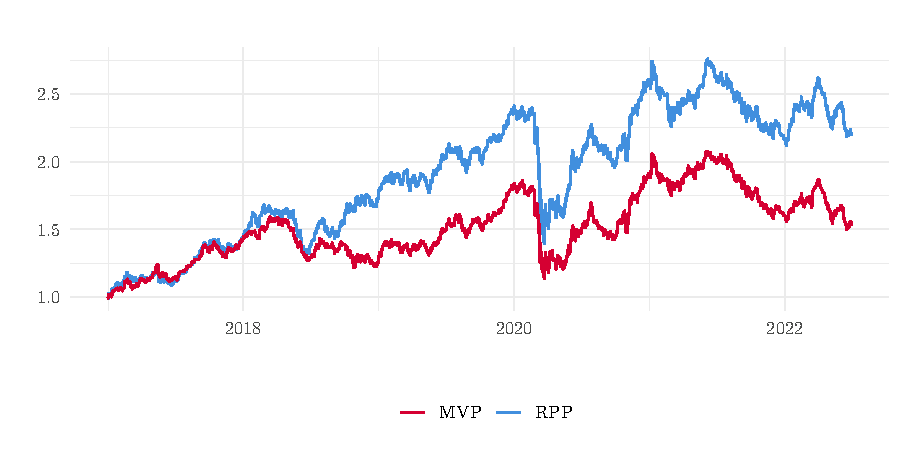
\includegraphics{figures/retornoRPPMVP.pdf}
	\caption{Total Return of MVP and RPP from Jan17 to Jun22.}
	\label{fig:retornoRPPMVP}
\end{figure}

We remind that, after 2020 due to the COVID-19 pandemic, the volatility of all assets has exploded, and we may observe that the RPP performed (135\% fo gain) much better than the MVP (79\% of gain) on the period between January 2017 and December 2019. From January 2020 to June 2022, MVP has an accumulated loss of $15.2\%$ while RPP reduced the loss to $6.8\%$.

\begin{figure}[H]
	%\begin{adjustwidth}{2.2cm}{2.2cm}
	\begin{subfigmatrix}{2}
		\subfigure[Jan17 $-$ Dez19]{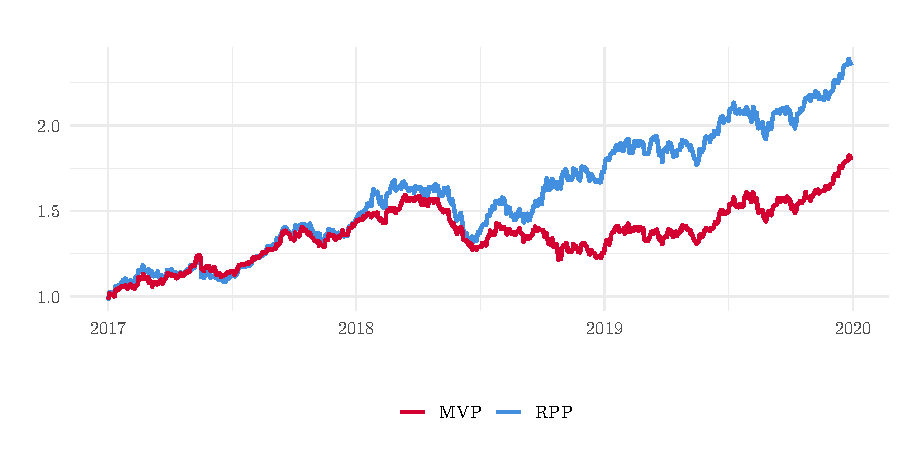
\includegraphics{figures/retornoRPPMVP1.pdf}}
		\subfigure[Jan20 $-$ Jun22]{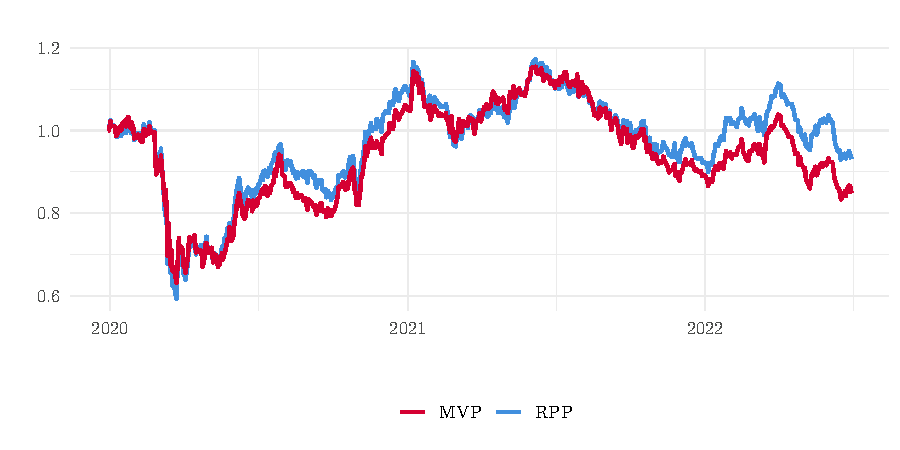
\includegraphics{figures/retornoRPPMVP2.pdf}}
	\end{subfigmatrix}
	\caption{Accumulated Return of MVP and RPP.}
	\label{fig:retornoRPPMVP12}
	%\end{adjustwidth}
\end{figure}

In this study, the RPP had a superior performance when compared to the MVP, both in high and low moments. Clearly, this study is not conclusive, it is just an example of the use of Algorithm~\ref{Alg:GeneralSeach}.


% Let $f(x;b)$ be the function defined by:
% \[
% f(x;b) = \sum_{i=1}^n \big(\mathcal{RC}_i(x) -b_i\mathcal{R}(x)\Big)^2
% \] and the following optimization problem
% \begin{eqnarray}\label{eq:MinProb}
% \min_{x\geq \textbf{0}}\, \{f(x;b)\}; \\
% 	\mbox{s.t. }\left\{
% 	\begin{aligned}\nonumber
% b_i \geq 0, \\
% x_i \geq 0, \\
% {\bf 1}^\top b =1, \\
% {\bf 1}^\top x =1.
% 	\end{aligned}
% 	\right.
% \end{eqnarray}

% If $x^\star$ is the solution to the problem (\ref{eq:MinProb}) and
% $f(x^\star;b)=0$, so $x^\star$ is also system solution
% (\ref{eq:SisNLin}). 


% Roncalli (2013) shows that under the hypothesis that $b_i>0$ the RB portfolio is the solution of the following optimization problem:
% \begin{eqnarray}\label{eq:MinProb}
% \min_{x\geq \textbf{0}}\, \{\mathcal{R}(x)\}; \\
% 	\mbox{s.t. }\left\{
% 	\begin{aligned}\nonumber
% \sum_{i=1}^n b_i \ln(x_i) \geq c, \\
% x_i \geq 0, \\
% {\bf 1}^\top x =1.
% 	\end{aligned}
% 	\right.
% \end{eqnarray}


% In the Gaussian case, when asset returns have a Normal distribution, we can consider $\mathcal{R}(x)=\sigma^2(x)$ and the system (\ref{eq:SisNLin}) reduces to
% \begin{eqnarray}\label{eq:SisGauss}
% x_i (\Sigma x )_i = b_i x^\top \Sigma x,\\
% 	\mbox{s.t. }\left\{
% 	\begin{aligned}\nonumber
% b_i \geq 0, \\
% x_i \geq 0, \\
% {\bf 1}^\top b =1, \\
% {\bf 1}^\top x =1.
% 	\end{aligned}
% 	\right.
% \end{eqnarray}
% for $i=1,2,\dots,n$.


% Setting $w=x/\sqrt{x^\top \Sigma x}$, the equation $x_i (\Sigma x )_i = b_i x^\top \Sigma x$ is equivalent to $w_i(\Sigma w)_i =b_i$, or, in vector form
% \[
% \Sigma w = b^\top/w.
% \]

% Observe that the convex function
% \[
% f(w)= \frac{1}{2}w^\top \Sigma w - b^\top log(w)
% \]
% has a gradient equal to
% \[
% \nabla f(w) = \Sigma w - b^\top/w
% \]
% and the system (\ref{eq:SisGauss}) can be reformulated by the following optimization problem
% \begin{eqnarray}\label{eq:GaussProb}
% \min_{x\geq {\bf 0}}\,\Big\{\frac{1}{2}w^\top \Sigma w - b^\top \log(w)\Big\};  \\
% 	\mbox{s.t. }\left\{
% 	\begin{aligned}\nonumber
% 		\mathbf{1}^\top x=1 & \\
% 		\mathbf{0}\leq x \leq \mathbf{1}
% 	\end{aligned}
% 	\right.
% \end{eqnarray}


% whose optimality condition is $\nabla f(w) = 0$ or $\Sigma w = b/w$ which is precisely the solution of the system (\ref{eq:SisGauss}).



